\subsection{Validazione e collaudo}
\textit{\textbf{Periodo}: dal 2021-04-09 al 2021-05-10}

L'inizio di questa fase coincide con data della Revisione di Qualifica e si conclude con la scadenza della Revisione di Accettazione.

\subsubsection{Attività}

\begin{itemize}
\item \textbf{Incremento e verifica documenti}: vengono realizzate le aggiunte necessarie ai documenti e le eventuali correzioni provenienti dalle segnalazioni del committente o da analisi interne. I documenti in questione sono:
\begin{itemize}
\item \NdP{};
\item \AdR{};
\item \PdQ{};
\item \PdP{};
\item Glossario;
\item \MU{};
\item \MM{}.
\end{itemize}
\item \textbf{Validazione e collaudo}: viene completato il prodotto in base a requisiti mancanti, indicazioni del proponente o analisi interne. Vengono inoltre eseguiti tutti i test per validare e collaudare il prodotto finale.\\ Gli incrementi individuati nella sezione \S{3.2} vengono, in questa fase, raggruppati a due a due. Il motivo è dato dal fatto che essi prevedono solo correzioni o aggiunte minime di funzionalità, il che risulta in un carico di lavoro minore rispetto alle due fasi precedenti. Inoltre gli incrementi, in questo caso, possono essere svolti in contemporanea da diversi membri del gruppo (per lo stesso motivo notato precedentemente);
\item \textbf{Consolidamento}: viene realizzata la presentazione da esporre in sede di Revisione di Accettazione.
\end{itemize}

\subsubsection{Periodi}

\begin{itemize}
\item \textbf{Periodo 1}: \textit{dal 2021-04-09 al 2021-04-15}. \\
Se necessario, verranno corretti i documenti realizzati nella fase di progettazione di dettaglio e codifica.
\item \textbf{Periodo 2}: \textit{dal 2021-04-15 al 2021-05-03}. \\
Verrà eseguita l'attività di validazione e collaudo. In contemporanea verranno incrementati e completati i manuali iniziati nella fase precedente. Di seguito vengono riportati i periodi individuati per i singoli incrementi:
\begin{itemize}
\item \textbf{Incremento 1 e 2}: \textit{dal 2021-04-17 al 2021-04-21};
\item \textbf{Incremento 3 e 4}: \textit{dal 2021-04-21 al 2021-04-25}.
\end{itemize}
Il periodo si conclude con la consegna del materiale per la Revisione di Accettazione;
\item \textbf{Periodo 3}: \textit{dal 2021-05-03 al 2021-05-10}. \\
Viene svolta l'attività di consolidamento. Il periodo si conclude con la Revisione di Accettazione.
\end{itemize}

\subsubsection{Diagramma di Gantt}

\begin{figure}[H]
\centering

\centerline{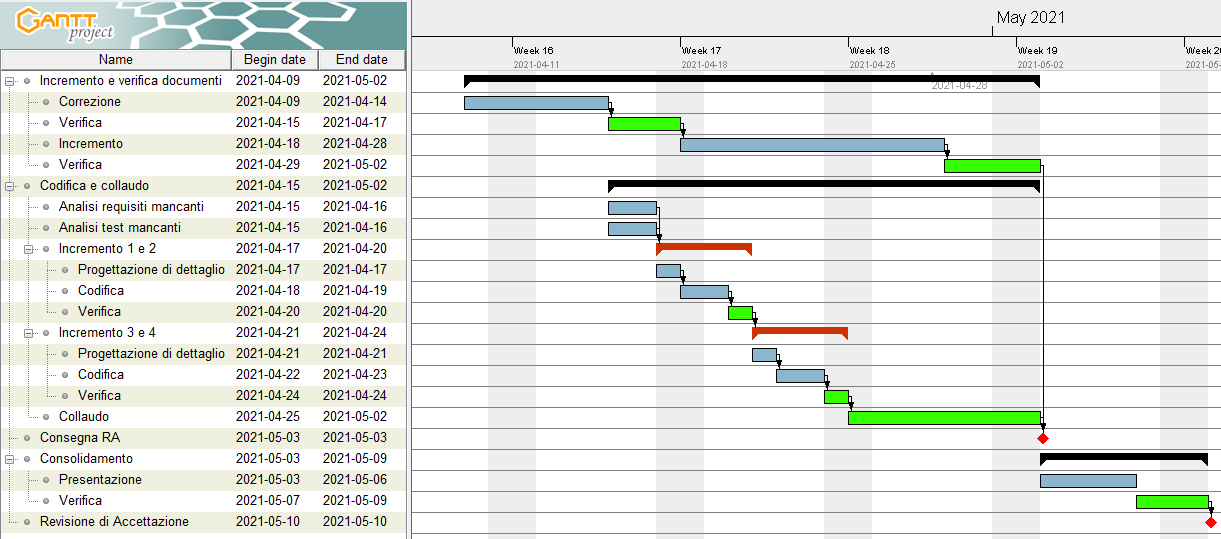
\includegraphics[scale=0.6]{res/Pianificazione/Gantt/verifica}}
\caption{Diagramma di Gantt per il periodo di validazione e collaudo}
\end{figure}